\section{Method}
\label{sec:method}

\subsection{Task, simulator and oracle}
\label{sec:task}

% \dnotedone{done: merged into one Method section, task setup first}{consider unifying 3 and 4 to one Method Section. maybe easier to understand if 4 comes before 3?}
A session is an English text conversation between a therapist policy and
a simulated patient who is ambivalent about a health behavior.
% \dnotedone{answered: cites Yosef et al. 2024 and the PTO paper}{ref some kfir paper?}
% 2026-10-07 (review round 4): the persona prompts are credited as adapted (the two uncooperative
% clauses were rewritten for this study; Appendix D.4 quotes them).
The patient is simulated by
\texttt{gpt-4o-mini} conditioned on one of \textbf{96} persona system prompts, the exhaustive
enumeration of $2\ \text{gender} \times 3\ \text{cooperation} \times 2\ \text{problem} \times
2\ \text{duration} \times 2\ \text{prior attempts} \times 2\ \text{age}$ of
\citet{yosef2024assessing}, as used in \citet{baruch2025pto} but with the two uncooperative clauses
rewritten here to make the patient more adversarial (Appendix~\ref{app:prompts}). A session runs
until the patient closes it or a cap of 49 utterances after the scripted opening is reached; most
close earlier, and the untrained therapist's sessions average 28.5 utterances. The therapist is the
pretrained, not instruction-tuned, \texttt{Llama-3.2-1B} under a fixed counselor system prompt,
trained with LoRA adapters, responses capped at 200 tokens (all setting parameters in
Table~\ref{tab:config}). The oracle is the same \texttt{gpt-4o-mini} with JSON-schema-constrained
output; the \emph{training} reward is the mean of two of the evaluation instruments, Q1 and Q2,
written \QQ\ (\S\ref{sec:setup}).

% 2026-10-07 (review round 4, Lior): "Why MI" reduced to the term definitions (the motivation is
% the Introduction's); the Q1+Q2 justification moved into the Instruments paragraph.
\textbf{MI terms.} MI's target outcome is \emph{change talk}, the patient's own statements in favor
of change (``I guess it would feel like a relief not to be chained to it''), as against
\emph{sustain talk}, statements in favor of the status quo (``I like my routine''; both from
Appendix~\ref{app:example}) \citep{miller2013mi, moyers2016miti}. The therapist's tools are open
questions, \emph{affirmations} (comments on a specific strength or effort of the patient) and
\emph{reflections}, which restate what the patient said (\emph{simple}) or add meaning to it, such
as an inferred feeling (\emph{complex}).

\subsection{GRPO with look-ahead}
\label{sec:lagrpo}

Throughout, a \emph{turn} is one utterance by either speaker, a \emph{prefix} $c$ is a transcript
ending on a patient turn, $\oplus$ appends turns to a transcript, $\pi_n$ is the therapist policy
after $n$ training iterations ($\pi_0$ is the untrained model, which we call the \emph{Base}), and
$\pi$ is the policy being updated within an iteration ($\pi = \pi_n$ at its start). The patient simulator $P$ and the oracle
$O$ are fixed LLMs; $O$ returns a scalar MI score for a transcript. Figure~\ref{fig:schematic}
shows one group; Algorithm~\ref{alg:loop} (Appendix~\ref{app:repro}) states the whole loop.

% 2026-10-07 (review round 4, Lior): Figure 1 at column width; Algorithm 1 moved to Appendix D.
\begin{figure}[t]
\centering
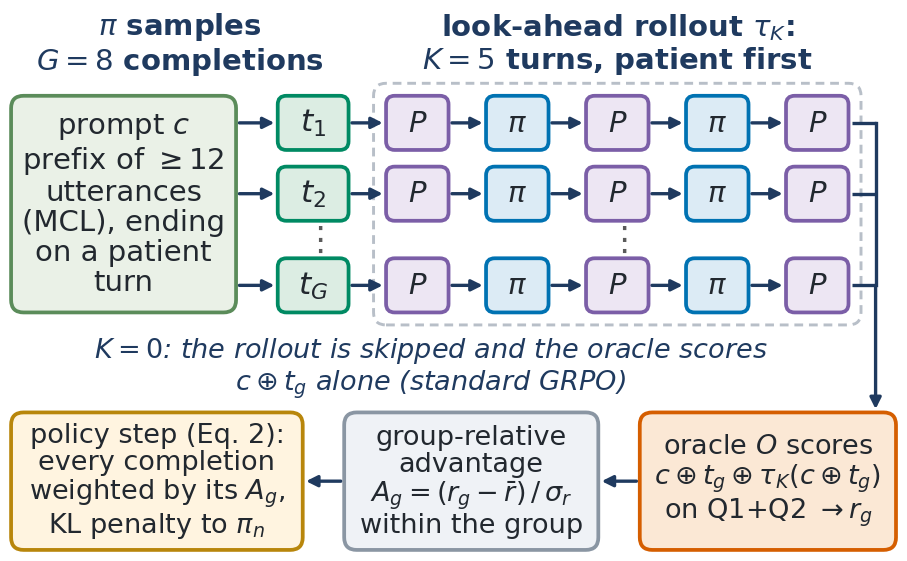
\includegraphics[width=0.48\textwidth]{figures/method_grpo_group.png}
\caption{One GRPO group under look-ahead. The policy samples $G{=}8$ completions $t_g$ of a
prompt $c$; the patient simulator $P$ and the policy $\pi$ being trained roll each forward $K$
turns; the oracle scores the extended transcript; the scores are standardized within the group,
and every completion, but no rollout turn, carries a gradient. At $K{=}0$ the oracle scores
$c \oplus t_g$ alone: standard GRPO.}
\label{fig:schematic}
\end{figure}

\textbf{The iterative loop.} Each training iteration starts from the current policy $\pi_n$,
which has 96 conversations with $P$, one per patient persona; each conversation is sliced after
every patient turn whose prefix has at least MCL utterances (the \emph{minimum context length}, 12
here; see below) to form the training prompts; the prompts of $5\%$ of the conversations are held
out as the trainer's validation split. For each prompt GRPO samples $G{=}8$ completions and
scores them; the policy takes one optimizer step per batch of 16 prompts (128 completions) on the
group-standardized scores, and after two epochs it is saved as $\pi_{n+1}$ and the loop repeats
with fresh conversations. The conversations that start an iteration double as the evaluation set
of $\pi_n$, and a generate-only pass after the last update evaluates the final policy, so every
policy from the Base $\pi_0$ to $\pi_{10}$ is evaluated; in the figures, iteration $n$ is $\pi_n$, and the Base pools the two runs' iteration-0 conversations (192).

\textbf{The look-ahead reward.}
% \dnotedone{rephrased: now names what the two runs differ in}{from what??}
The two runs differ in one design choice: whether a candidate turn is
rolled forward by a simulated $K$-turn look-ahead before it is scored, and hence which transcript
the oracle rewards. Let $\tau_K(x)$ be the $K$-turn rollout of a transcript $x$: $P$ replies, then
$\pi$, then $P$, and so on for $K$ turns, stopping early if the patient closes the session;
$\tau_0(x)$ is empty. Then
\begin{equation}
\label{eq:reward}
r_g \;=\; O\big(c \oplus t_g \oplus \tau_K(c \oplus t_g)\big).
\end{equation}
At $K{=}0$ the oracle scores the conversation so far, ending on the candidate, with nothing after it.
% \dnotedone{rephrased; cost clause cut, costs stay in Limitations}{[at the price of three [why? is this important?] patient-simulator calls and two policy generations per candidate and roughly twice the per-step wall-clock \ldots{} this all seems too AI. rephrase to make it clear and focus on what is interesting..]}
At $K{=}5$ it scores the candidate together with the five turns that follow it under the current
policy (the rollout uses the evaluation decoding, not the candidates' sampling temperature;
Table~\ref{tab:config}).
% \dnotedone{cut: heading and PTO comparison gone, one point kept here}{which transfer? }
A rollout is one sample from the
distribution of continuations, so $r_g$ is a one-sample Monte Carlo estimate of the candidate's
downstream value, with sampling noise from $P$ and $\pi$ added to the oracle's own; GRPO trains on
all $G$ candidates, so that variance enters every advantage.

\textbf{The update.} The step maximizes the GRPO objective of \citet{shao2024deepseekmath}: the
per-token surrogate
\begin{equation}
\label{eq:grpo}
\ell_{g,i} = \min(\rho_{g,i} A_g,\,\bar{\rho}_{g,i} A_g) - \beta\,\mathrm{KL}_{g,i},
\end{equation}
averaged over the tokens of each completion and then over the group, where $\rho_{g,i}$ is the
$i$-th token's probability ratio between $\pi$ and the sampling policy, $\bar{\rho}_{g,i}$ its
clip to $[1{-}\epsilon, 1{+}\epsilon]$, and $\mathrm{KL}_{g,i}$ the per-token KL estimate to
$\pi_n$. Both runs make one update per sampled batch
(Table~\ref{tab:config}), so $\rho_{g,i}{=}1$ at the update, the clipping is inactive, and the
step is the advantage-weighted policy gradient over the group with the KL penalty.

\textbf{Minimum context length.} Training prompts are prefixes, so the oracle scores a partial
conversation while the evaluation scores a whole session.
% \dnotedone{done: cites Appendix C.1 and its new figure}{ref specific subsection and related figure}
In a pilot on an earlier configuration
of this task the oracle's ranking of very short prefixes agreed poorly with its ranking of the
completed sessions, so both runs discard prefixes shorter than MCL${=}12$. The Base's own
conversations show the same: the training oracle's score of a prefix ranks them as their
full-session scores do in $74\%$ of pairs at two utterances, $85\%$ at twelve and $98\%$ at fifty
(Appendix~\ref{app:faithfulness}, Figure~\ref{fig:faithfulness}).

\subsection{Evaluation design}
\label{sec:setup}

\textbf{Instruments.} Evaluation uses eight instruments, each scored by an LLM judge from
the full transcript (Table~\ref{tab:instruments}; items and prompts in
Appendix~\ref{app:instruments}).
\dnotedone{done here, and now also in the intro (the paragraph presenting the method) and in the Discussion (before the Conclusion)}{need to talk about this - here briefly but also in intro and/or discussion - I guess the excuse is following Yosef et al .. }
Q1 and Q2 are the LLM-evaluator questionnaires of \citet{yosef2024assessing}, 5 and 17
patient-perspective Likert items on session satisfaction and on alliance and relational
communication, built and validated there for LLM evaluation of simulated MI sessions and shown to
separate levels of therapist expertise; this is why their mean, \QQ, is the training reward, as
for PTO \citep{baruch2025pto}. The Working Alliance Inventory, Short Revised (WAI-SR;
\citealp{hatcher2006waisr}) and the Client Satisfaction Questionnaire (CSQ-8;
\citealp{larsen1979csq}) are published patient-report instruments, and MI-SAT is a six-item
intervention-satisfaction survey adapted for this task. The other three code behavior: a
Motivational Interviewing Treatment Integrity (MITI~4.2.1) coder \citep{moyers2016miti4,moyers2016miti}
whose four global ratings are averaged; patient change talk (PCT), the share of change talk among
the change and sustain talk in the utterance coder's patient codes (next paragraph), the
patient-side outcome MI aims at; and an MI-inconsistent-behavior coder (MICI; acts per therapist
turn, lower is better) that counts the MI-inconsistent codes of the Motivational Interviewing Skill
Code (MISC) 2.5 \citep{houck2010misc} plus an over-praise code of our own. \QQ\ is thus both the
optimization target and a reported outcome; the six instruments outside the reward are not
optimized directly, and the held-out judge (below) checks the shared judge.

\textbf{The utterance coder.} The eight instruments are session-level aggregates. For
\S\ref{sec:therapist}--\ref{sec:patient} we also label every utterance: an LLM \emph{utterance
coder} assigns each therapist utterance one code, its dominant function in the terms of
MITI~4.2.1 and the MISC~2.5 (open question, closed question, simple reflection, complex
reflection, affirmation, non-specific praise, giving information, persuasion with or without
permission, seeking collaboration or emphasizing autonomy, confront, other), and each patient
utterance one code (change talk, sustain talk, neutral), in transcript order
(Appendix~\ref{app:coder}). Affirmation follows the MITI definition, a comment on a specific client
strength or effort; non-specific praise is coded separately, the distinction the MITI manual draws
when it lists ``I am really proud of you'' as not an affirmation. We count open questions,
reflections, affirmations and seeking collaboration as MI-consistent, and non-specific praise,
persuasion and confront as MI-inconsistent (our grouping; Appendix~\ref{app:coder}).
% \dnotedone{rephrased: now says we read the patient's reply}{[say what the patient said next ?\textasciitilde{}]}
% 2026-10-07 (review round 4): the transcript-order sentence and the MITI "MI-adherent" comparison
% moved to Appendix D.3.

\textbf{Judges.} Two LLMs score the conversations, and each does two jobs: it fills in the
instruments for a whole conversation, and it runs the utterance coder, which also gives PCT. The \textbf{training
oracle} (\primaryjudge, which also plays the patient and gave the training reward) is the main
judge: the results in the body are its readings. The \textbf{held-out judge} (\heldoutjudge, a
different model family that never touched training) re-scores everything as a check; the body
reports it in Table~\ref{tab:endpoint} and in one sentence per results section, and the rest is in
Appendix~\ref{app:heldout}.

\textbf{The two runs.} The runs are a controlled pair: their tracked run configurations differ in
exactly two fields, the look-ahead depth and the look-ahead sub-batch size, which only sets how
many rollouts advance together. Everything else, from $G{=}8$, KL $\beta{=}0.01$ and the sampling
temperature to the seed, the oracle and the persona set, is identical (Table~\ref{tab:config}),
except that one resume changed the KL reference for the second half of the $\Kf$ run's first
iteration (Appendix~\ref{app:repro}); the horizon enters only through $r_g$. We name the runs by
their horizon, \Kz\ (turn-level reward) and \Kf\ (look-ahead reward); from \S\ref{sec:reward} on,
``the \Kf\ policy'' is the therapist a run produces and ``the \Kf\ run'' the training that produced
it.

\textbf{Evaluation and statistics.} Every policy is scored on all eight instruments and coded
utterance by utterance for all 96 personas by both judges. All contrasts are
\textbf{persona-paired} (personas are reshuffled every iteration, so pairing is on the recovered
persona identity), with Wilcoxon signed-rank tests, Cohen's \dz\ (the mean persona-paired
difference divided by its standard deviation), bootstrap intervals and Holm correction for
multiple comparisons within each family of tests. We call a contrast \emph{significant} when its
Holm-corrected $p$ is below .05; a contrast repeated at every iteration is corrected across the
ten iterations, and the contrasts of an endpoint table across its rows, per judge. The two judges'
questionnaire scores are not on a common scale (on \QQ\ the held-out judge scores 1.2--1.8 points
lower), so they are compared only through contrasts and never averaged.
